\documentclass[12pt]{article}
\usepackage{amsmath,amssymb,amsthm}
\usepackage{epic}
\usepackage{eepic}
%\usepackage{hyperref}
\usepackage{listings}
\usepackage{float}
\usepackage{graphicx}
\usepackage{fancyhdr}
\usepackage{color}
\usepackage{enumitem}
\usepackage[letterpaper, margin=1in]{geometry}
\usepackage{cleveref}

\newcommand{\C}{\mathbf{C}}
\newcommand{\R}{\mathbf{R}}
\newcommand{\Q}{\mathbf{Q}}
\newcommand{\Z}{\mathbf{Z}}
\newcommand{\N}{\mathbf{N}}
\newcommand{\E}{\mathbf{E}}
\newcommand{\B}{\mathbf{B}}
\newcommand{\F}{\mathbf{F}}
\newcommand{\U}{\mathbf{U}}
\newcommand{\V}{\mathbf{V}}
\newcommand{\J}{\mathbf{J}}
\newcommand{\x}{\mathbf{x}}
\newcommand{\y}{\mathbf{y}}
\newcommand{\z}{\mathbf{z}}
\newcommand{\Sb}{\mathbf{S}}
\newcommand{\Cs}{\mathscr{C}}
\newcommand{\As}{\mathscr{A}}
\newcommand{\I}{\textnormal{\textbf{I}}}
\newcommand{\Id}{\dot{\textnormal{\textbf{I}}}}
\newcommand{\Top}{\textnormal{\textbf{Top}}}
\newcommand{\hTop}{\textnormal{\textbf{hTop}}}
\newcommand{\Groups}{\textnormal{\textbf{Groups}}}
\newcommand{\Set}{\textnormal{\textbf{Set}}}
\newcommand{\Xib}{\mathbf{\Xi}}
\newcommand{\Sym}{\text{Sym}}
\newcommand{\prid}[1]{\langle #1 \rangle}
\newcommand{\apoly}[1]{a_{#1} + a_{#1}x+ a_{#1}x^2 + \cdots + a_{#1}x^n}
\newcommand{\dist}{\textnormal{dist}}
\newcommand{\ti}[1]{\textit{#1}}
\newcommand{\tb}[1]{\textnormal{\textbf{#1}}}
\newcommand{\es}{\emptyset}
\newcommand{\sst}{\subset}
\newcommand{\ssteq}{\subseteq}
\newcommand{\func}[3]{#1: #2 \to #3}
\newcommand{\inte}[1]{\textnormal{int}(#1)}
\newcommand{\bdr}[1]{\textnormal{bdry}(#1)}
\newcommand{\ifff}{if and only if }
\newcommand{\st}{such that }
\newcommand{\wrt}{with respect to }
\newcommand{\tspace}[1]{\text{T}_#1}
\newcommand{\mathdash}{\hbox{-}}
\newcommand{\diam}[1]{\textnormal{diam}(#1)}
\newcommand{\setst}{\hspace{1mm} | \hspace{1mm} }
\newcommand{\supp}{\textnormal{support}}
\newcommand{\clos}{\textnormal{closure}}
\newcommand{\rel}{\textnormal{rel }}
\newcommand{\Hom}{\textnormal{Hom}}
\newcommand{\obj}{\textnormal{obj}}
\newcommand{\varlisto}[2]{#1_1,#1_2,\ldots,#1_{#2}}
\newcommand{\varlistz}[2]{#1_0,#1_1,\ldots,#1_{#2}}
\newcommand{\finv}[2]{#1^{-1}(#2)}
\newcommand{\disu}{\rotatebox[origin=c]{90}{$\models$}}
\newcommand{\rank}{\textnormal{rank }}
\newcommand{\card}{\textnormal{card }}
\newcommand{\im}{\textnormal{im }}
\newcommand{\cls}{\textnormal{cls }}
\newcommand{\rev}{\textnormal{rev }}
\newcommand{\defeq}{\mathrel{\stackrel{\makebox[0pt]{\mbox{\normalfont\tiny def}}}{=}}}
\newcommand{\Err}{\textnormal{Err}}
\newcommand{\Var}{\textnormal{Var}}
\newcommand{\Ev}{\textnormal{E}}

\renewcommand{\epsilon}{\varepsilon}


\newtheorem*{solution*}{Solution}
\newtheorem{theorem}{Theorem}[section]
\newtheorem{corollary}[theorem]{Corollary}
\newtheorem{proposition}{Proposition}[theorem]
\newtheorem{lemma}[theorem]{Lemma}
\theoremstyle{definition}
\newtheorem*{definition}{Definition}
\newtheorem*{remark}{Remark}
\newtheorem*{remarks}{Remarks}


\renewcommand\qedsymbol{$\blacksquare$}

\author{Luke Meszar}
\date{September 15th, 2017}
\title{CSCI 5622 Homework 1}

\begin{document}
	\thispagestyle{empty}
	
	% --- Header Box --- %
	\newlength{\boxlength}\setlength{\boxlength}{\textwidth}
	\addtolength{\boxlength}{-4mm}
	
	\begin{center}\framebox{\parbox{\boxlength}{\bf
				Machine Learning \hfill Homework 1\\
				CSCI 5622 Fall 2017 \hfill Due Time Sep 15, 2017\\
				Name: Luke Meszar \hfill CU identitykey: lume0018
		}}
	\end{center}
	\section{K-nearest Neighbor (40pts)}																																									
	\begin{solution*}\leavevmode
		\begin{enumerate}[label=\arabic*.,font=\upshape]
			\item \textnormal{What is the role of the number of training instances to accuracy? }
			\begin{figure}[H]
				\centering
				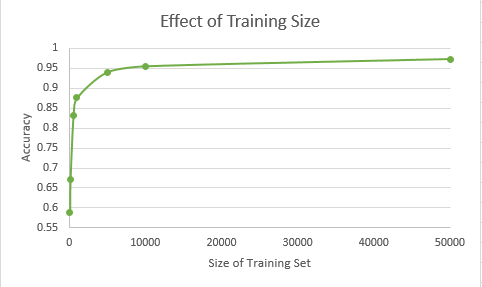
\includegraphics[scale=0.6]{AccuracyVsTrainingSize}
				\caption{Training data size vs. accuracy with $k$ = 3}
				\label{fig:sizevsaccuracy}
			\end{figure}
		
			We see from \Cref{fig:sizevsaccuracy} that the accuracy increases as the size of the training set increases. We notice there is a quick increase in accuracy when we change the size of the training set for small training set sizes. For instance, between size $50$ and size $100$, the accuracy increases from $58$\% to $67$\%. When the training size is already large, making it bigger doesn't have much effect on the accuracy. As an example, between size $10,000$ and $50,000$, there is only about a $2$\% increase in accuracy. Looking at the graph, it seems that around a training set size of $10,000$ is where the diminishing returns begin.
			\item \textnormal{What numbers get confused with each other most easily?}
			
			I tested with $k = 3$ and a limit of $500$ and $5000$. For a limit of $500$, the most misclassified number was a $9$ being confused for a $4$ with a $155$ misclassifications. The $2$nd most misclassified number was a 9 being confused with a $7$ with $95$ misclassifications. There was a tie for the third most misclassified number, each with $63$ misclassifications. These were a $7$ being confused with a $2$ and and a $3$ being confused with an $8$. 
			
			When the training set size was increased to $5000$, the most misclassified number was still a $9$ being confused with $4$. However, the number of times this confusion happened when down to $55$.
			\item \textnormal{What is the role of $k$ to training accuracy?}
			
			Three tests were run. One where the size of the training data was $500$, one where the size was $5000$ and one where the size was $10000$. The value of $k$ varied over odd values between $1$ and $13$. The results were as follows:
			
			\textnormal{
				\begin{table}[h]
					\centering
					\begin{tabular}{cc}					
						$k$ & Accuracy \\\hline
						1 & 0.8458 \\
						3 & 0.8311 \\
						5 & 0.8033 \\
						7 & 0.7986\\
						9 & 0.7900\\
						11 & 0.7825 \\
						13 & 0.7690 
					\end{tabular}
					\caption{Accuracy vs $k$ for training set size of 500}
				\end{table}	
			}
			
			
			\textnormal{
			\begin{table}[h]
				\centering
				\begin{tabular}{cc}					
					$k$ & Accuracy \\\hline
					1 & 0.9388 \\
					3 & 0.9401 \\
					5 & 0.9341 \\
					7 & 0.9307\\
					9 & 0.9308\\
					11 & 0.9271 \\
					13 & 0.9246 
				\end{tabular}
			\caption{Accuracy vs $k$ for training set size of 5000}
			\end{table}	
		}
	
		\textnormal{
			\begin{table}[h]
				\centering
				\begin{tabular}{cc}					
					$k$ & Accuracy \\\hline
					1 & 0.9513 \\
					3 & 0.9544 \\
					5 & 0.9492 \\
					7 & 0.9461\\
					9 & 0.9441\\
					11 & 0.9417 \\
					13 & 0.9411 
				\end{tabular}
				\caption{Accuracy vs $k$ for training set size of 10000}
			\end{table}	
		}
			
			The most accurate $k$ changes depending on the size of the training set. When the size of the training set is $500$, then the most accurate is $k = 1$. When the size of the training set is either $5000$ or $10000$, then the most accurate is $k = 3$.
			
			\item \textnormal{In general, does a small value for $k$ cause ``overfitting'' or ``underfitting''?}
			
			In general, a small value of $k$ will cause underfitting. When $k$ is small, the algorithm only sees a few neighbors and cannot make a accurate prediction and won't perform well on the training data. As the size of $k$ increases, then the algorithm learns the training data too well and it will be unable to predict well on new data. 
		\end{enumerate}
	\end{solution*}
	
	\section{Cross Validation (30pts)}
	\begin{solution*}\leavevmode
		\begin{enumerate}[label=\arabic*.,font=\upshape]
			\item \textnormal{What is the best } k \textnormal{chosen from 5-fold cross validation with ``\texttt{--limit 500}''? } 
			At \textnormal{\texttt{--limit 500}} the best $k$ is $3$ with accuracy $0.8311$.
			\item \textnormal{What is the best } k \textnormal{chosen from 5-fold cross validation with ``\texttt{--limit 5000}''? }
			
			At \textnormal{\texttt{--limit 5000}} the best $k$ is $1$ with accuracy $0.9388$.
			\item \textnormal{Is the best } k \textnormal{consistent with the best performance} k \textnormal{in problem 1?}
			
			The optimal $k$ is different for size $500$ and $5000$ as found in problem $1$. This is not surprising since the cross validation breaks up the training data differently so the testing conditions are not the same as in problem $1$. 
		\end{enumerate}
	\end{solution*}
	
	\section{Bias-variance tradeoff (20pts)}
	\begin{proof}
		From the lecture, we know that the general form for bias-variance tradeoff is as follows: 
		\[\Err(x_0) = \sigma^2_\epsilon + \left[\Ev(h(x_0))-f(x_0)\right]^2 + \Var(h(x_0)).\]
		We begin by computing $\text{Bias}^2$:
		\begin{align*}
		\left[\Ev(h(x_0))-f(x_0)\right]^2 &= \left[\Ev\left(\frac{1}{k}\sum_{l=1}^{k}(f(x_l)+\epsilon_l)\right)-f(x_0)\right]^2 \\
		&= \left[\frac{1}{k}\Ev\left(\sum_{l=1}^{k}f(x_l)\right)+\Ev\left(\sum_{l=1}^{k}\epsilon_l\right)-f(x_0)\right]^2\\
		&= \left[\frac{1}{k}\left(\sum_{l=1}^{k}f(x_l)\right)-f(x_0)\right]^2 \text{ assuming fixed nearest neighbors and } \Ev(\epsilon) = 0.
		\end{align*}
		Then, we compute the Variance:
		\begin{align*}
		\Var(h(x_0)) &= \Var\left(\frac{1}{k}\sum_{l=1}^{k}(f(x_l)+\epsilon_l)\right) \\
		&= \frac{1}{k^2} \Var\left(\sum_{l=1}^{k}(f(x_l)+\epsilon_l)\right) \\
		&= \frac{1}{k^2}\left(\sum_{l=1}^{k}\left(\Var(f(x_l))+\Var(\epsilon_l\right)\right) \\
		&= \frac{1}{k^2}\left(0+k\sigma^2_{\epsilon}\right) \text{ assuming fixed nearest neighbors and } \Var(\epsilon) = \sigma^2_\epsilon \\
		&= \frac{\sigma^2_\epsilon}{k}.
		\end{align*}
		Combining these two steps, we get that
		\[\Err(x_0) = \sigma^2_\epsilon + \left[\frac{1}{k}\left(\sum_{l=1}^{k}f(x_l)\right)-f(x_0)\right]^2 + \frac{\sigma^2_\epsilon}{k}.\]
	\end{proof}
\end{document}